\chapter{Background}

  This chapter provides a background to our works that exists. These background are either derived from looking into kernel code or 
  are parts of existing design details.
  
  \section{Memory management between processes in Linux}
  
    Memory is allocated/deallocated in terms of pages in a Linux operating system. Memory management in Linux is done using techniques like 
virtual memory, demand paging, swapping caching etc. They separate between the memory needed by a process and the memory physically 
allocated on the RAM. The OS creates a large virtual address space for each process. In this section we focus on how memory is managed 
between processes or a group of processes. We mainly focus on how memory is assigned and reclaimed between them.  
  
    \subsection{Memory pages used by a process}
      Memory used by processes are divided into 3 types of pages	
      \begin{enumerate}	
	\item Anonymous Pages: Pages those which are not associated with any files on disk. They are process memory pages and have a virtual
	address (VA) associated with it.
	\item Page cache pages: Are an in-memory representation of a files on the disks but don't have a VA associated with it.	
	\item Mapped pages: Are also an in-memory representation of a file on the disk but also have a VA associated with it.
      \end{enumerate}
  
    \subsection{Memory allocation}
      When the process needs memory to be allocated, Linux decides the how this memory is going to be allocated physically on the RAM. The 
process/ application does not see in physical RAM addresses. It only sees virtual addresses from the virtual space assigned to each process.
The OS uses a page file located on the disk to assist with memory requests in addition to the RAM. Less RAM means more pressure on the Page 
file. When the OS tries to find a piece of memory that's not in the RAM, it will try to find in the page file, and in this case they call it 
a page miss. The actual physical memory allocated (RSS) to a process depends on how much free memory is available in the system. On free 
memory becoming freshly available in the system, the OS tries to equally distribute the available memory to all processes that are 
demanding for more memory.

    \subsection{Memory reclamation without container support}
      When the system memory starts to get tight, the kernel can free memory by cleaning up its own internal data structures - reducing 
the size of the inode and dentry caches however most pages in the system are user process pages. Hence the kernel, in order to accommodate 
current demands for user pages, must find some existing pages to toss out. A proper balance between anonymous and page cache pages must be 
maintained for the system to perform well. Kernel offers a knob called swappiness, that specifies how much favor anonymous versus page 
cache pages while reclamation. The default value for swappiness favors the eviction of page cache pages. 
      
      The system maintains two LRU lists to evict pages in the system commonly referred as \textit{LRU/2 algorithm}, one active list 
      containing all the pages that were recently used and another inactive list which contains all the pages that weren't used recently. 
      One pair (active and inactive) for anonymous pages and one pair for page cache pages. The kernel favors reclamation from page cache 
      pages over anonymous pages and inactive pages over active pages and iterates these lists to satisfy reclamation requests there by 
      trying to maximize application performance while satisfying requests.

%%%%%%%%%%%%%%%%%%%%%%%%%%%%%%%%%%%%%%%%%%%%%%%%%%%%%%%%%%%%%%%%%%%%%%%%%%%%%%%%%%%%%%%%%%%%%%%%%%%%%%%%%%%%%%%%%%%%%%%%%%%%%%%%%%%%%%%%%%%%%%%%%      

  \section{Containers}
    
        Container in simple terms can be defined as, 
  
    \begin{center}
      \textit{``Container is a process or set of processes grouped together along \\ with its dependent resources into a single logical OS 
entity. \\It enables multiple isolated user-space instances on a host machine.''} 
    \end{center}
    
    Containers \cite{manual} are built as an extension to the existing operating system and not as an independent system. Container 
provides virtualization of isolated user spaces at an OS-level and hence containers executing on a host machine reuse the functionalities of 
the host kernel. This makes it better by reducing redundant kernel pages as used in VMs but comes at the cost of containers only of host OS 
type to execute on a system.

     \begin{figure}
      \centering
      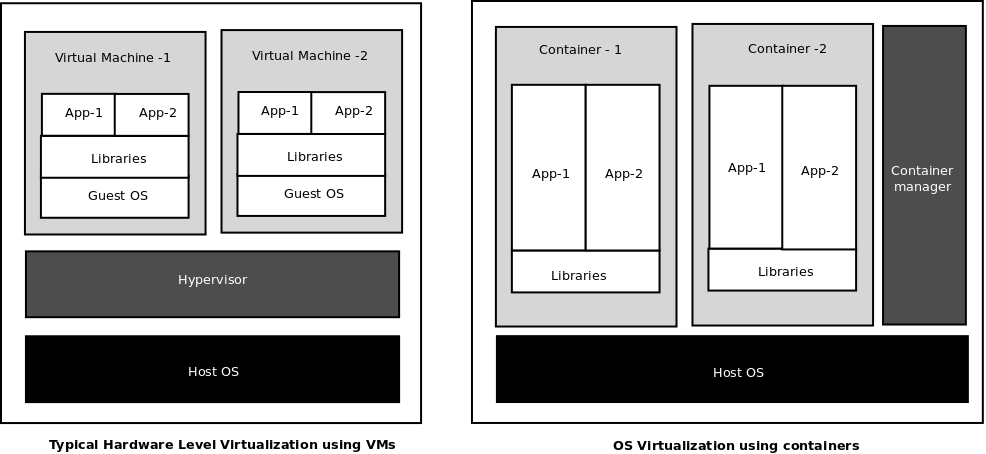
\includegraphics[width=1\textwidth]{images/background/container_vs_vm.png}
      \caption{Difference between a VM and Container}
      \label{img:difference}
    \end{figure}

A high level difference between a VM and containers can be seen in Fig~\ref{img:difference}. The biggest advantage of using containers over 
virtual machines is that they provide much lesser performance overheads. Containers are usually managed by container managers, which are 
entities similar to how Hypervisors are to VMs. Container managers are shipped by different organizations like Docker \cite{docker}, LXD 
\cite{lxd}, OpenVZ \cite{kolyshkin2006virtualization} etc. All container managers makes use of 3 Linux kernel components and combine 
them to form the building structure. The deploy their own controllers on top of this. 
    
    \begin{enumerate}
      \item Control Groups: Used for resource accounting and control
      \item Namespaces: Resource isolation among resources provisioned to different users on the same system
      \item Disk Images: The disk image which provides the ROOTFS for a container to execute. It contains the distribution related 
packages, libraries, and application programs.
    \end{enumerate}
    
    For the purpose of this discussion, we would focus on control \cg{} (\cg{}) as this provides the mechanism to control resources 
which includes performing memory management.

%%%%%%%%%%%%%%%%%%%%%%%%%%%%%%%%%%%%%%%%%%%%%%%%%%%%%%%%%%%%%%%%%%%%%%%%%%%%%%%%%%%%%%%%%%%%%%%%%%%%%%%%%%%%%%%%%%%%%%%%%%%%%%%%%%%%%%%%%%%%%%%%%
  
    \subsection{Control groups}
      
      \begin{figure}
	\centering
	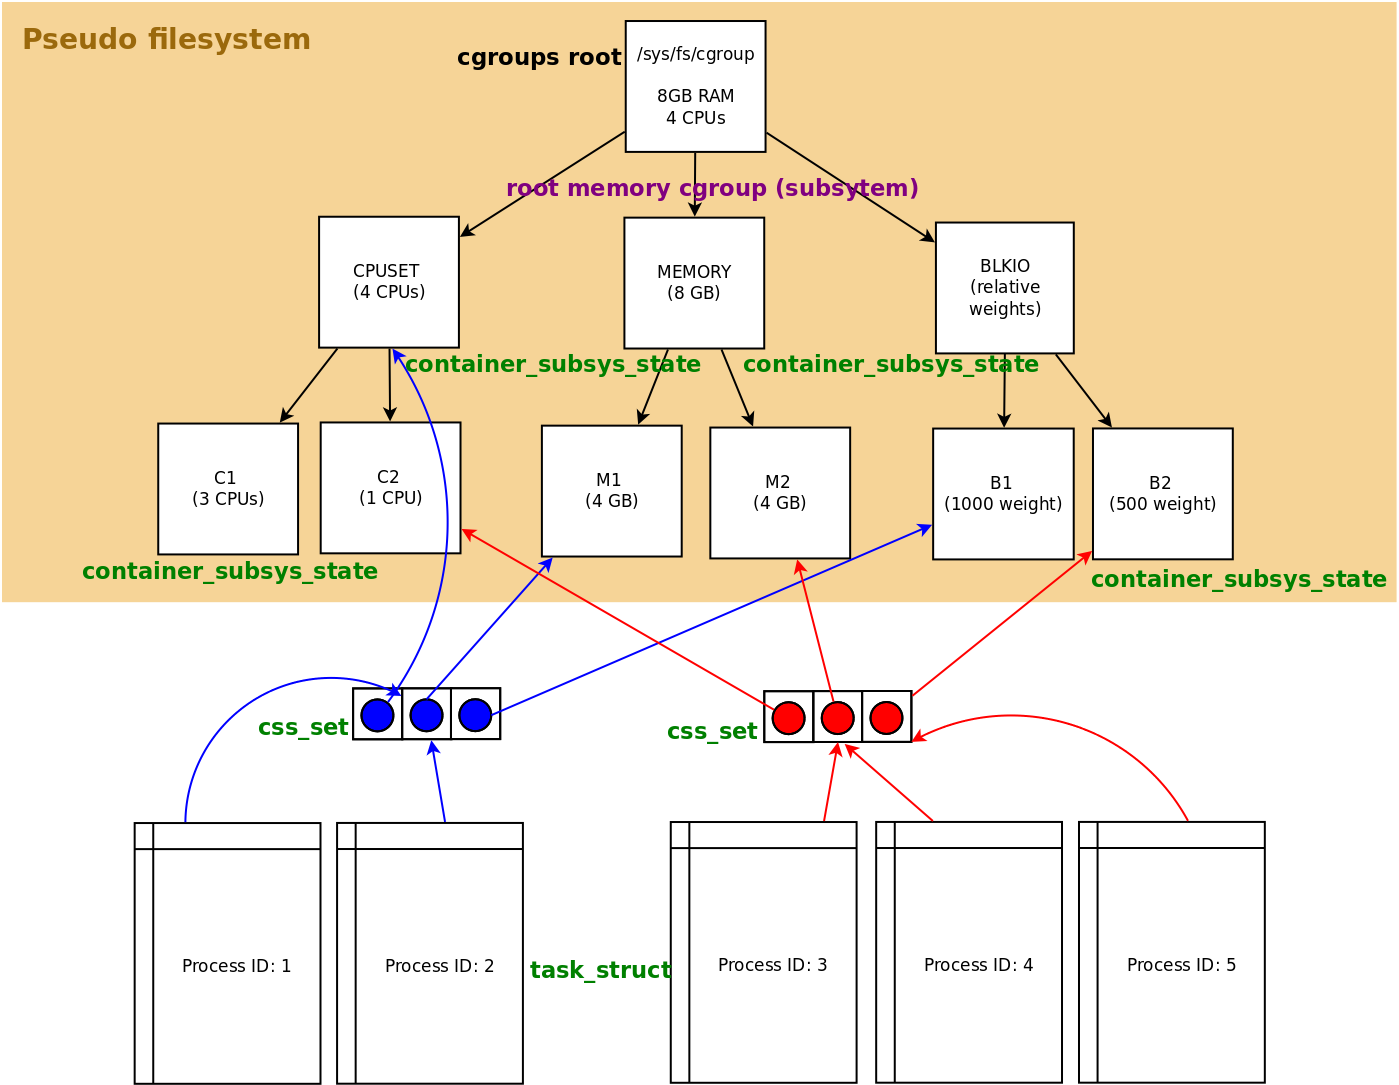
\includegraphics[width=1\textwidth]{images/background/control_groups.png}
	\caption{Control groups illustration using 3 controllers, Source:\cite{manual}}
	\label{img:cgroup}
      \end{figure}
      
      A solution to process group control and accounting was proposed by Google in 2007 which was originally called Generic Process 
Containers \cite{menage2007adding} and was later renamed to Control Groups (\cg{}), to avoid confusion with the term Containers. A 
cgroup/subsystem refers to a resource controller for a certain type of CPU resource. Eg- Memory cgroup, Network cgroup etc. It is derives 
ideas and extends the process-tracking design used for cpusets system present in the Linux kernel. There are 12 different 
\cg{}/subsystems, one for each resource type classified.

      For the purpose of our discussion we will stick to subsystem as the terminology referring to individual resource control and cgroup 
to refer a cgroup node in hierarchy. The Linux kernel by default enables most subsystems. The overheads introduced by \cg{} are 
negligible. Most subsystems follow their own hierarchy for their individual resource. The Linux exposes Pseudo file systems as userspace 
APIs to interact with them.

      Fig~\ref{img:cgroup} illustrates a minimalistic outline of a \cg{} hierarchy with 3 subsystems mounted in a system onto their own 
  hierarchies. The three subsystem mounted are - memory, cpuset and blkio and are mounted at \texttt{/sys/fs/\cg{}/}. Memory root cgroup 
of   8GB is divided into two \cg{} M1 and M2 of 4GB each. cpuset root cgroup of 4CPUs is divided into two \cg{} C1 and C2 of 3CPUs and 
1CPU respectively. blkio root cgroup of is divided into two \cg{} B1 and B2 of 1000 and 500 as relative weights respectively. Every 
process   which attaches itself to the same set of subsystems are referred by a single \texttt{css\_set} which in turn points to the 
cgroup node the   process is attached to. In the Fig, processes 1,2 attach itself to the blue \texttt{css\_set} and 3,4,5 to the red one. 
The \texttt{css\_set} in turn has pointers to \texttt{container\_subsys\_state} that is one for each cgroup. Notice how the blue 
\texttt{css\_set} points to the   root cpuset cgroup there by assigning it all the CPUs in the system which is also a valid and 
default value to attach processes.
      
      \subsubsection{Memory \cg{}}
	
	Memory subsystem use a common data structure and support library for tracking usage and imposing limits using the "resource 
counter". Resource controller is an existing Linux implementation for tracking resource usage. Memory cgroup subsystem allocates three 
\texttt{res\_counters}. The three of them are described below.

      \textbf{i. Accounting:} Accounting memory for each process group. Keeps track of pages used by each group. Pages can be classified 
into four types. 
      \begin{itemize}
	\item Anonymous: Stack, heap etc.
	\item Active: Recently used pages
	\item Inactive: Pages read for eviction
	\item File: Reads/Writes/mmap from block devices
      \end{itemize}
	
      \textbf{ii. Limits:} Limits can be set on each \cg{}. Limits are of two types - soft and hard. Soft limit is the limit up to which 
the system guarantees availability. Hard limit is the limit up to which the system tries to accommodate, but cannot guaranty this if 
system is under memory pressure. Limits can be set in terms of byte for,
      \begin{itemize}
	\item Physical memory
	\item Kernel memory
	\item Total memory (Physical + Swap)
      \end{itemize}

      \textbf{iii. OOM:} Out Of Memory killers are used to kill processes or trigger any other such event on reaching hard limit by a 
process group. 

	More about memory management using memory subsystem in the Linux kernel shall be described in the coming section.
	
	\paragraph{Memory reclamation with \cg{}}
	
      \begin{figure}
	\centering
	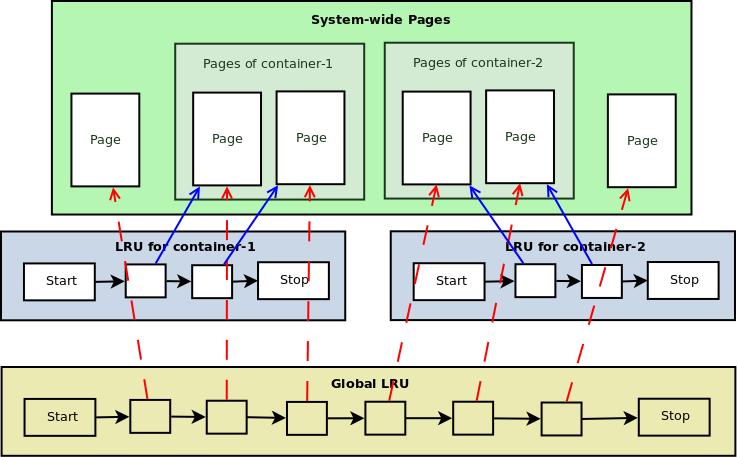
\includegraphics[width=0.8\textwidth]{images/background/page_mapping.png}
	\caption{Mapping of pages to LRU lists}
	\label{img_page_mapping}
      \end{figure}
      
      Most recent Linux kernels that are even skipped through stable Linux distribution support Linux containers. They provide the 
following set of knobs to provision containers - Hard limit, Soft Limit, OOM Control, Swappiness to name a few important ones. Hard limits 
can further be specified in terms of process, kernel and tcp memory utilization. However, with respect to reclamation we focus on soft 
limits here.
    
      The following section describes the existing policy based on theoretical readings and looking upon Linux kernel code. The current 
system-wide policy incorporates memory reclamation keeping in mind the memory \cg{}. Reclamation can broadly occur in two situations,
      \begin{enumerate}
	\item \textbf{System-Wide (Global) Reclamation:} When the system is under memory pressure when all/most of its pages are occupied
	\item \textbf{Container Specific (Local) Reclamation:} When only a particular of the container is under pressure due to exceeding 
its hard limit
      \end{enumerate}
      
      For the purposes of our problem, we focus on System-Wide Reclamation. It must be remembered that System-wide reclamation can again 
broadly occur in two situations,       
      \begin{enumerate}
	\item \textbf{Synchronous:} When system is under memory pressure due to new page requests and not enough free pages available
	\item \textbf{Asynchronous:} System clears up memory routinely when free
      \end{enumerate}         
      
      Both Synchronous and Asynchronous global reclamation ultimately end up taking a similar path for memory reclamation, with little 
differences when it comes to regions to reclaim from and how much to reclaim. A kernel function call trace for system-wide reclamation is 
described in Fig~\ref{img_call_trace}. It shows how sync and async requests are ultimately mapped to the same set of function calls.

      \begin{figure}
	\centering
	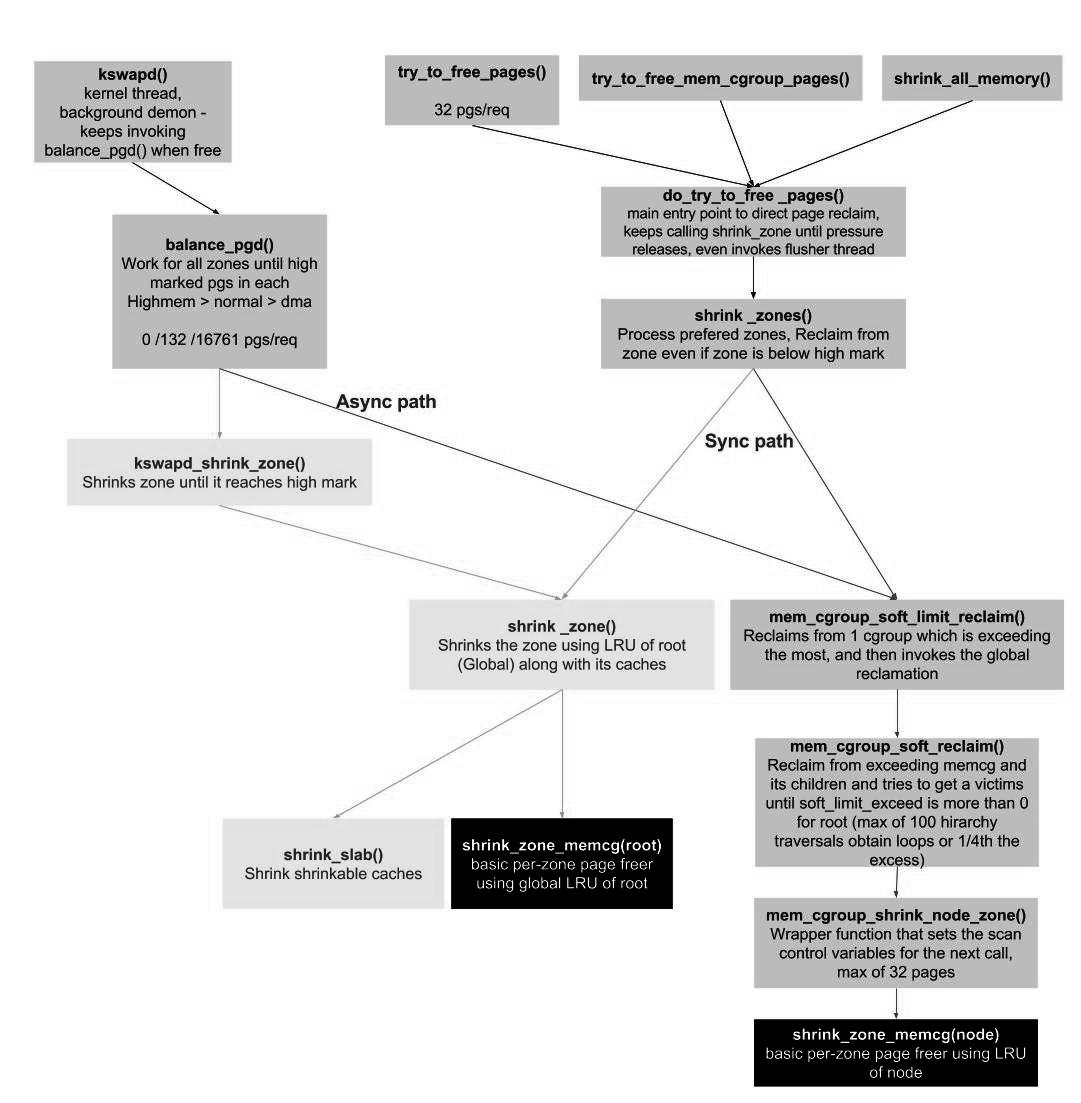
\includegraphics[width=1\textwidth]{images/background/reclamation_call_trace.jpg}
	\caption{Kernel Function Call Trace for System-Wide Reclamation}
	\label{img_call_trace}
      \end{figure}

      \begin{figure}
	\centering
	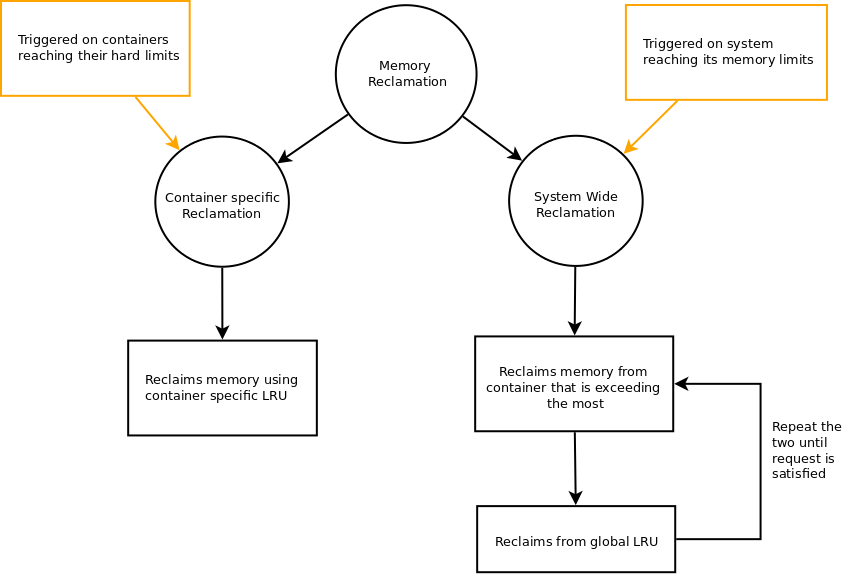
\includegraphics[width=0.8\textwidth]{images/background/high_level_Reclamation.png}
	\caption{Existing policy for Memory Reclamation}
	\label{img_high_level}
      \end{figure}  
      
      As shown in Fig~\ref{img_page_mapping}, in recent Linux kernels a LRU (LRU/2, but LRU used for simplicity) list is stored for every 
container created also there is a Global LRU list which contains the pages of all processes in the system (including in the ones in a new 
container). All processes are by default put into the default container and hence its pages are a part of the global LRU.  Once a process is 
moved to a specific container, its pages also become a part of its local per container LRU list also.
    
      An container (Memory cgroup) when has its soft limit set, has a value called excess computed for it at every container node. The 
system internally makes use of a RBTree to store the exceeds. The exceed is computed at \texttt{mem\_cgroup\_update\_tree()} at regular 
intervals using the formula,
      
	  \begin{center}
	    \begin{equation}
	      Excess = Usage - SoftLimit
	    \end{equation}
	  \end{center}
      
      \pagebreak
      
      \noindent Two types of reclamations after the global reclamation policy used currently, 
      
      \begin{itemize}
       \item \textbf{Soft Memory Reclamation (SMR):} is the one specific to \cg{} where container which exceeds its 
soft limits by the most is reclaimed from using the per container based LRU. It internally also reclaims from all its child containers.  
       \item \textbf{Global LRU reclamation policy (GLR):} reclaims based on the global LRU list in which all processes in the system are a 
part of
      \end{itemize}     
      
      The existing reclamation policy is illustrated as a flow chart in Fig~\ref{img_high_level}. In simple terms the global reclamation 
policy is a combination of both Soft Memory Reclamation and the native global LRU based reclamation. The reclamation algorithm tries to 
maximize most of the requested reclamation from SMR and prefers GLR only when requests aren't being satisfied by SMR.

      All above container specific memory reclamation patterns were derived based on theoretical readings and looking upon Linux kernel 
code. We need to establish the correctness our hypotheses, and understand the existing system and how it impacts applications running 
inside containers in a native container setup and derivative cloud setup. Hence the coming sections describes the empirical analysis to 
do the same.
      
  
  \section{Second chance cache for derivative clouds}
  
    \dd{}\cite{doubledecker} is a second cache caching framework developed to support derivative clouds. It's initial intent was to tackle the
    problem of configuring hypervisor caches in a derivative cloud environment. 
    
    \dd{} provides a second chance caching framework for Linux+KVM+LXC.
    \dd{} is built upon existing the existing \tmem{} second cache caching framework for Linux. There have been implementations\cite{venkatesan2014ex} of \tmem{} 
    to support a per-VM partitioning schema. \dd{} builds upon this framework by providing a per-container partitioning framework.
    
    \noindent The following are a comprehensive list of features supported by \dd{},
      \begin{enumerate}
	\item Supports a \textbf{two level configurable caches}. These partitions are either in-memory or at the SSD. 
	\item A cache partition can be configured on a per-VM basis by the native cloud provider at the hypervisor.
	\item The cache partitioned at the VM-level can further be partitioned by an derivative cloud provider inside the VM on a \textbf{per-container basis}.
	\item Cache supports a \textbf{resource conserving nature}, where any cache that is underutilized is provisioned to other applications at need
	more cache.
	\item Exclusive caching at all levels.
      \end{enumerate}
      
   \paragraph{Architecture}
    \label{sec:double_decker_architecture}
    
      \begin{figure}
	\centering
	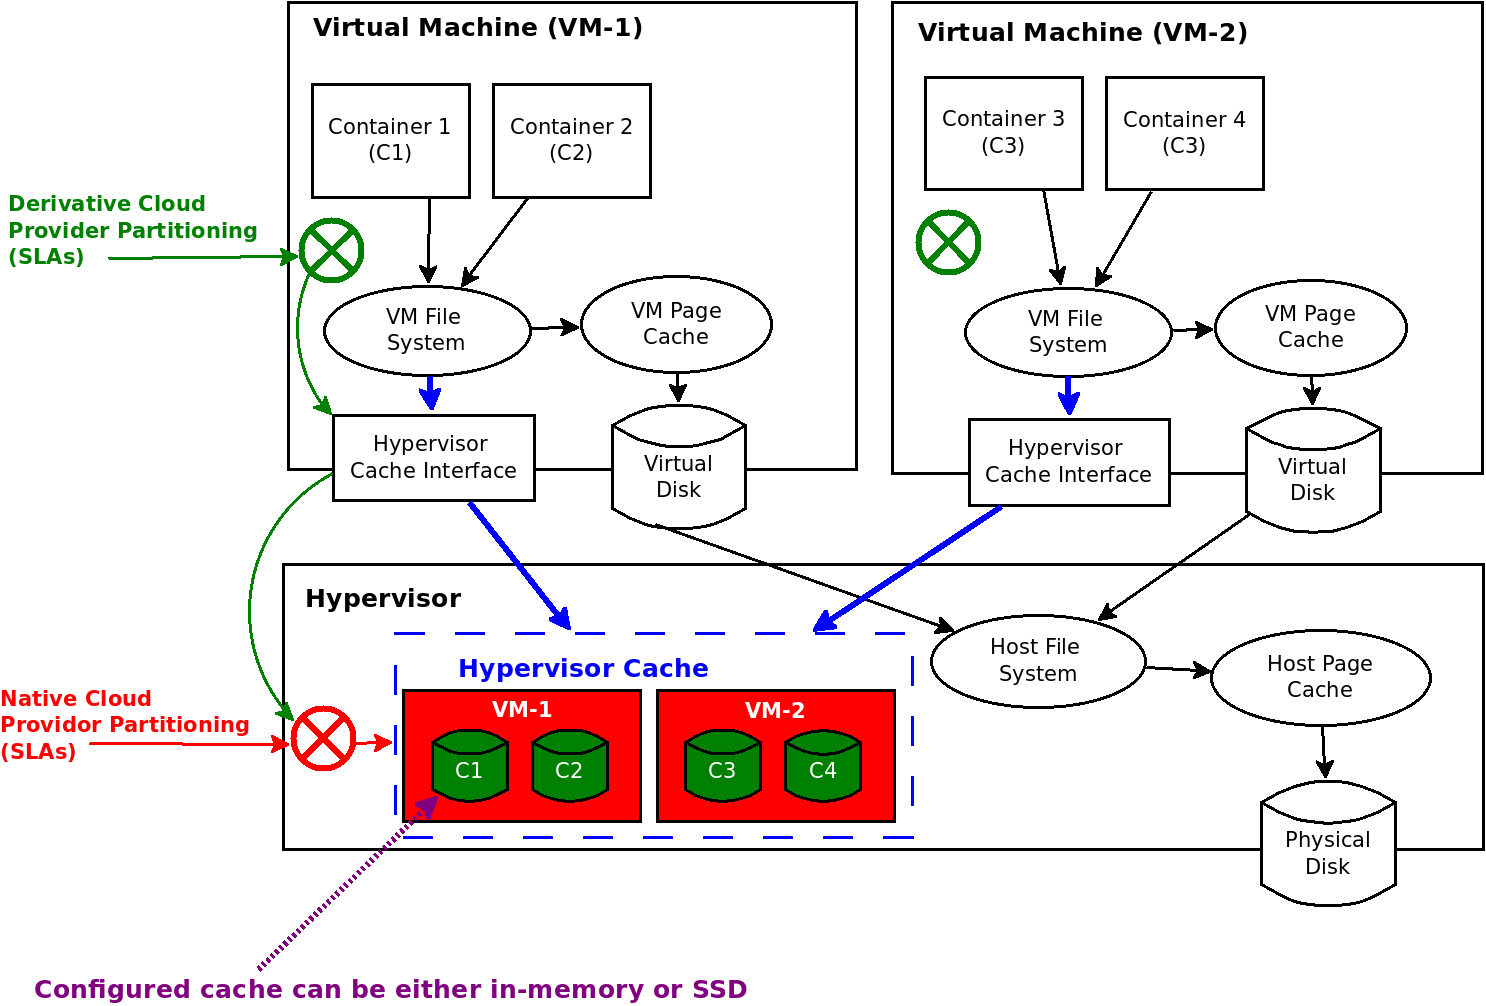
\includegraphics[width=1\textwidth]{images/background/double_decker.png}
	\caption{\dd{} architecture: second cache caching for derivative clouds}
	\label{img:doube_decker_architecure}
      \end{figure}
      
	The architecture for \dd{} is illustrated in Fig~\ref{img:doube_decker_architecure}. The hypervisor caches are initially partitioned on a per-VM
	basis by the native cloud provider at the hypervisor. Now, each VM cache partition can be further subdivided by the derivative cloud provider 
	on a per container basis. Provisioning is done in-terms of \textit{Relative Weights}. The relative weight for an container would map to the
	actual cache partition as given below,
	  
	  \begin{center}
	    \begin{equation}
	    \label{eq:cache_allocation}
	      Container Cache Allocation = ( \frac{Relative Weight of Container}{Total Weight of all Containers} ) * Cache Allocated for VM
	    \end{equation}
	  \end{center}
	  
	Similarly is the cache partition for each VM calculated but instead of using the VM cache allocation, we would be using the entire 
	host cache configuration. The cache is partitioned based on a higher level SLA requirements at each of the cloud provider. This SLA could
	be fixed for a particular container using a higher level policy. 
	  
    \paragraph{Internals}
    \label{sec:double_decker_internals}
    
      \begin{figure}
	\centering
	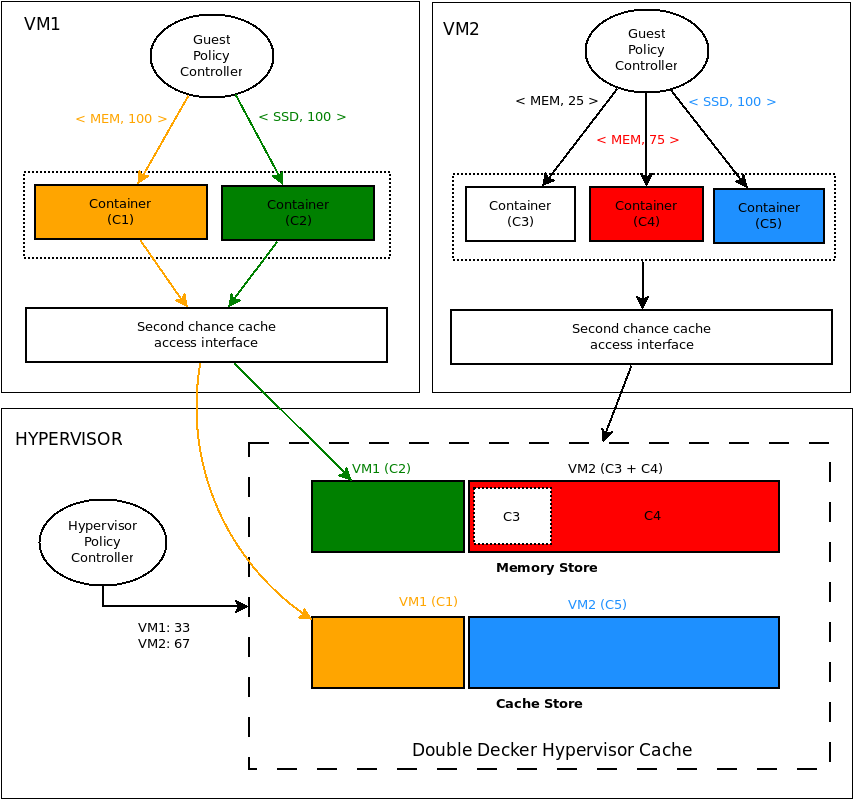
\includegraphics[width=0.75\textwidth]{images/background/single_level_implementation.png}
	\caption{\dd{} internals}
	\label{img:doube_decker_internals}
      \end{figure}
	  
	The Fig~~\ref{img:doube_decker_internals} describes the \tmem{} implementation overview of double decker. Each container is configured using a
	relative weight parameter as described in Section~\ref{sec:double_decker_architecture}. There is pool created for each configured container cache. This
	pool represents an abstract design component which contains all the pages for a particular container are present in. 
	There are several data structures which make up  for the \tmem implementation, however the most crucial one is a per pool tree structure that keeps 
	track of all put objects.
	
	\dd{} is built upon existing the existing \tmem{} second cache caching framework for Linux as mentioned earlier. In specific it only works as a second
	cache only clean (not dirty) disk backed pages. It doesn't cache anonymous (pages with VA mappings) or dirty disk backed pages. This ensures a simple 
	form of consistency in case of system failure. 
	
	Inserts into the cache are referred to as \textit{PUTS} and accesses to these objects are referred to as \textit{GETS}. Cleaning up of pages are referred
	to as \textit{FLUSHES}. Evictions in this triggered when the cache is full, and the application (VM followed by container) that is most exceeding it's 
	limits are targeted first. Evictions are based on a simple LRU eviction algorithm for now. However any eviction algorithm is pluggable with this implementation.
  
    
  
      

      